\chapter[Os dados]{Os dados}
\label{sec:dados}

Neste capítulo serão tratadas as características dos dados usados neste trabalho.

\section{Seleção dos dados}

Os dados foram processados e extraídos no desenvolvimento do projeto Victor\footnote{Victor é o Projeto de Pesquisa \& Desenvolvimento de aprendizado de máquina (machine learning) sobre dados judiciais das repercussões gerais do Supremo Tribunal Federal - STF.}. Dessa forma, eles são os mesmos que apresentados por  \citeonline{da_silva_document_2018} e \citeonline{braz_document_2018}. Além disso, há confiabilidade nos rótulos dos documentos processados, pois estes foram rotulados por especialistas em direito.

As 5 categorias de documentos Agravo de Recurso Extraordinário, Acordão, Despacho de Admissibilidade, Recurso Extraordinário e Sentença foram escolhidas por serem as peças avaliadas pelo STF para definir se um processo se encaixa em algum tema. Os pricipais motivos obtidos através de conversas informais com representantes do STF foram:

\begin{itemize}
    \item Acordãos possuem uma síntese de alto nível da tese jurídica tratada no processo, que é de extrema importância para avaliação do STF.
    \item Sentença é o documento de menor peso, avaliado apenas em alguns casos específicos nos quais não foi possível determinar o tema com as outras 4 peças e busca-se por mais informações da tese jurídica tratada no processo.
    \item Despacho de Admissibilidade é utilizado principalmente para averiguar se o processo está em acordo com as regras de submissão do CPC (Lei n.º 13.105/2015).
    \item Recurso Extraordinário é a principal peça avaliada, pois ela é o artefato gerado para ser encaminhado ao STF. Neste artefato, tem-se os motivos pelos quais recorreu-se ao julgamento de segunda instância, incluindo o(s) artigo(s) da CF \citeyear{brasil_constituicao_1988} que foram infringidos.
    \item Agravo de Recurso Extraordinário é utilizando quando presente no processo, pelo mesmo motivo que o RE.
    \item Outro é a categoria para agrupar o restante das peças que não se encaixam em nenhuma das anteriores.
\end{itemize}

\section{Extração dos textos}

\begin{figure}[h]
	\centering
    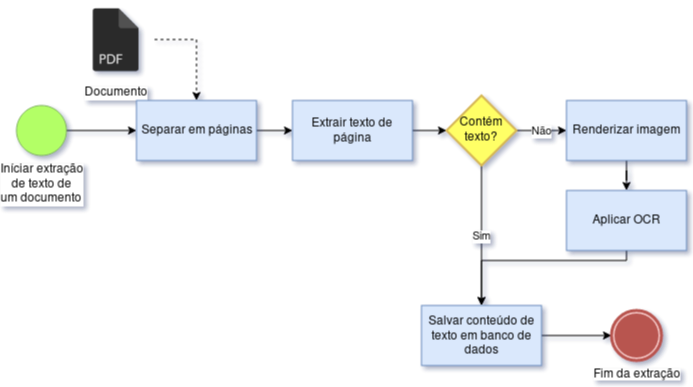
\includegraphics[keepaspectratio=true,scale=0.6]{figuras/extracaoDados}
    \caption[Procedimentos para extração de textos]{Procedimento para extração de textos. São aceitos volumes ou peças separadas. O texto extraído é salvo em uma base de dados. Fonte: \citeonline[p. 2]{da_silva_document_2018}}
    \label{fig:extracaoDados}
\end{figure}

O STF disponibilizou os processos e suas peças no formato PDF. Nos arquivos recebidos há volumes e peças já separadas.

As etapas necessárias para realizar a extração de documentos estão representadas na Figura \ref{fig:extracaoDados}, onde utilizou-se da ferramenta XpdfReader\footnote{Executou-se os comandos \textbf{pdftotext} e \textbf{pdftopng}. Disponível em: \url{https://www.xpdfreader.com/pdftotext-man.html}. Acesso em: 17-06-2018.} para extrair o texto das páginas de um PDF que estava em formato digital ou digitalizado com uma camada de texto.

Quando encontrada uma página sem texto, transformou-se esta em uma imagem para, em seguida, aplicar um reconhecedor ótico de caracteres (do inglês \textit{Optical Character Recognition} OCR).

\section{Tratamento dos textos}

Utilizou-se apenas parte dos dados para realizar a análise. Fez-se a limpeza utilizando expressões regulares \cite{goyvaerts_regular_2012} a fim de:

\begin{itemize}
	\item Remover caracteres especiais, tais como: \# @ $\backslash n$ 0xCE;
    \item Remover números misturados com letras;
    \item Remover números;
    \item Capturar leis, artigos e decretos;
    \item Remover espaços em branco;
    \item Remover e-mail e \textit{link}.
\end{itemize}

Em seguida, aplicou-se as técnicas de radicalização, normalização \cite{singh_text_2016} e remoção de palavras recorrentes \cite{manning_introduction_2008}. Ao analisar os dados, detectou-se a presença de nomes próprios, símbolos e sequências de caracteres sem sentido para a língua portuguesa, \textit{latim} e para o contexto Jurídico Brasileiro.

Ao processar os dados, fez-se uma restrição no tamanho do vocabulário adquirido pelo modelo de transformação do texto ao invés de utilizar palavras pré-determinadas. isto devido à variabilidade de palavras com erros de OCR ser alta. Utilizou-se as palavras contidas nos próprios documentos pois elas podem ser representativas para este conjunto de texto, além de que os mesmos erros podem aparecer em outros documentos que sofreram o mesmo tratameno de digitalização.

Diferentemente do modelo de tratamento de dados para este contexto \cite{da_silva_document_2018}, não foi aplicado a normalização das palavras, ficando elas no formato final como apresentado na Tabela \ref{tab:palavrasSimbolos}.

% Além das palavras recorrentes, foram removidos nomes de pessoas e algumas palavras chaves específicas: 'elytho', 'neve', 'chenaud', 'tayrone', 'besen', 'youngéqyoung', 'sarubbi', 'balogh', 'pezarini', 'zezinho', 'intdo', 'izmailov', 'zotto', 'angelicoadvogados', 'limar', 'steiger', 'acidelma', 'vitoriar', 'tic', 'valcy', 'dadico', 'aloisia', 'itos', 'tendolo', 'rossol', 'catapani', 'cleudes', 'her', 'araçatuba', 'boeing', 'melar', 'rs', 'onaita', 'britar', 'ferreiro', 'licht', 'josé'.

% Os nomes de pessoas coletados para adicionar na remoção de palavras, foram obtidos através da mineração dos dados abertos do governo\footnote{Arquivo da data de Janeiro/2017 dos gastos diretos. Disponível em: \url{http://www.portaldatransparencia.gov.br/downloads/mensal.asp?c=FavorecidosGastosDiretos}. Acesso em: 17-06-2018}, com o procedimento do Apêndice \ref{sec:apendiceA}. 

\section{Características dos dados}

Como abordado na Seção \ref{sec:problema}, os rótulos das peças separadas dos volumes advindos do STF não são confiáveis. Por conta disso, houve um novo rotulamento destes documentos, classificando-os apenas em 5 categorias e Outros, apresentados na Tabela \ref{tab:categoriasPecas}.

A quantidade de documentos obtidos são apresentados na Tabela \ref{tab:categoriasPecas}. Nela, percebe-se que as peças de Agravo, Sentença, Petição de Agravo, Despacho de Agravo e Recurso Extraordinário não estão uniformemente distribuídas.

\begin{table}[ht]
	\centering    
	\caption[Amostras do conjunto de dados]{Amostras do conjunto de dados, contagem disponível em cada conjunto: Treino, Validação e Teste e seus respectivos totais nos conjuntos.}
    \label{tab:categoriasPecas}
	\begin{tabular}{|l|c|c|c|c|}
        \hline
        \textbf{Tipo} & \textbf{Treino} & \textbf{Validação} & \textbf{Teste} & \textbf{Total}\\ 
        \hline
        Agravo de Recurso Extraordinário &  640 & 183 & 92 & 915 \\
        \hline
        Acordão & 573 & 164 & 82 & 819 \\
        \hline
        Despacho & 388 & 111 & 55 & 554 \\
        \hline
        Outro & 1961 & 561 & 280 & 2802 \\
        \hline
        Recurso Extraordinário & 440 & 125 & 63 & 628 \\
        \hline
        Sentença & 767 & 219 & 110 & 1096 \\
        \hline
        \textbf{Total} & 4769 & 1363 & 682 & \textbf{6814} \\
        \hline

    \end{tabular}\par Fonte: \citeonline[p. 2]{da_silva_document_2018}
\end{table}

Após o tratamento dos dados, fez-se a remoção de  documentos com o mesmo conteúdo que tivessem classificações diferentes. As categorias que se confundiram foram as tuplas Outros e Acórdão, Agravo de Recurso Extraordinário e Recurso Extraordinário, Despacho e Outros, Acórdão e Sentença, e por último Petição de Agravo e Outros.

Foram feitos quatro tipos de processamentos nos dados coletados: a transformação em símbolos e o \textit{Bag Of Words}, com os dados crus e também pré-processamento. As análises dos documentos para o dado com a simples transformação em símbolos são apresentados na Tabela \ref{tab:metricasDocumentos}.

\begin{table}[ht]
	\centering    
	\caption[Métricas dos documentos]{Métricas dos documentos.}
    \label{tab:metricasDocumentos}
	\begin{tabular}{|l|c|c|}
        \hline
        \textbf{Nome} & \textbf{Sem pré-processamento} & \textbf{Pré-processado} \\
        \hline
        Menor número de símbolos & 10 & 20 \\
        \hline
        Maior número de símbolos & 945 & 790 \\
        \hline
        Média de símbolos por documento & 262,88 $\pm$ 116,93 & 145.83 $\pm$ 75.50 \\
        \hline
        Total de símbolos & 1.253.677 & 695.485 \\
        \hline
        Tamanho do vocabulário & 42.870 & 18.670 \\
        \hline
    \end{tabular}\par Fonte: elaboração própria.
\end{table}

Antes de treinar um modelo classificador, fez-se uma correlação entre as classes com o \textbf{BoW relativo}. Ou seja, o corpo de texto de cada tipo de documento foi concatenado, logo após, a contagem de palavras em cada tipo foi dividido pelo total de ocorrências dela em todos os documentos. Na Equação \ref{eq:bowRelativo}, o $i$ representa o tipo de documento e o $j$ representa a palavra pertencente ao dicionário. O $t$ representa todo o corpo textual.

\begin{equation}
\label{eq:bowRelativo}
	BoWrelative_{i,j} = \frac{BoW_{i,j}}{BoWt_{j}} \times 100
\end{equation}

A partir desse resultado, fez-se a correlação de \textit{spearman} para gerar uma matriz triangular. Os valores para o coeficiente de \textit{spearman} têm os intervalos entre $[-1,1]$, sendo a diagonal principal igual a 1. Os dados observados na Figura \ref{fig:correlacaoPecas} mostram que não há correlação entre os documentos, na qual o maior valor presente é a correlação entre Acórdão e a peça Despacho.

\begin{figure}[ht]
    \centering
    \begin{subfigure}[b]{0.45\textwidth}
        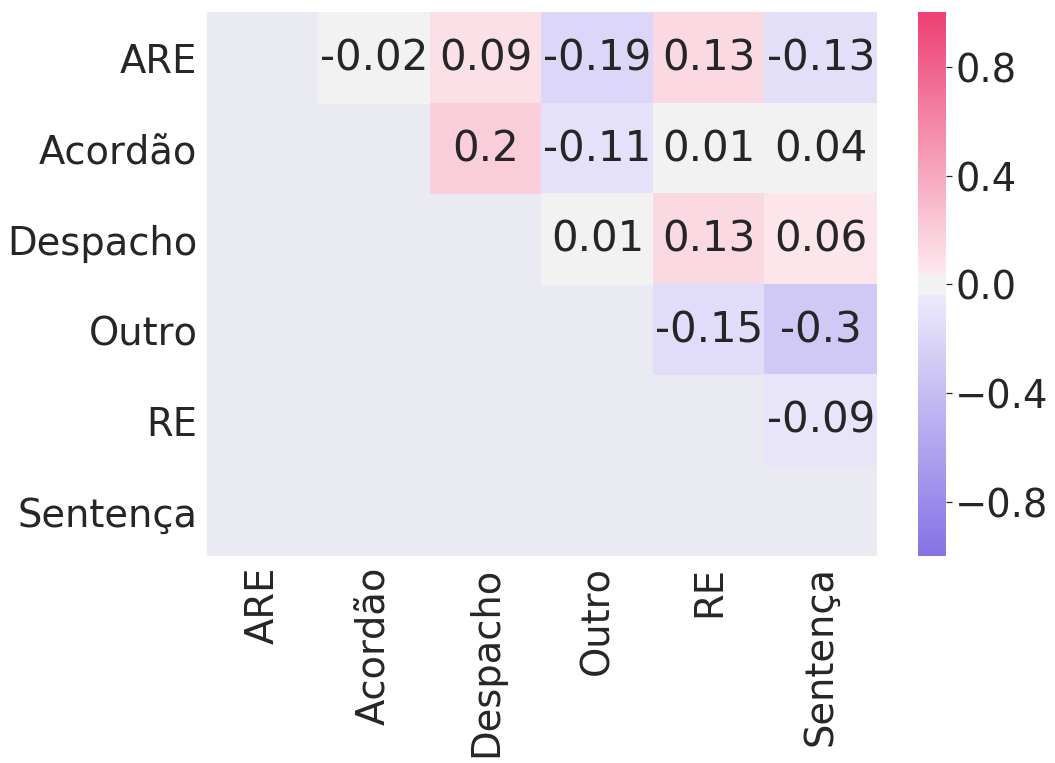
\includegraphics[width=\textwidth]{figuras/corr}
        \caption{Correlação do texto sem pré-processamento}
    \end{subfigure}\hfill
    \begin{subfigure}[b]{0.45\textwidth}
        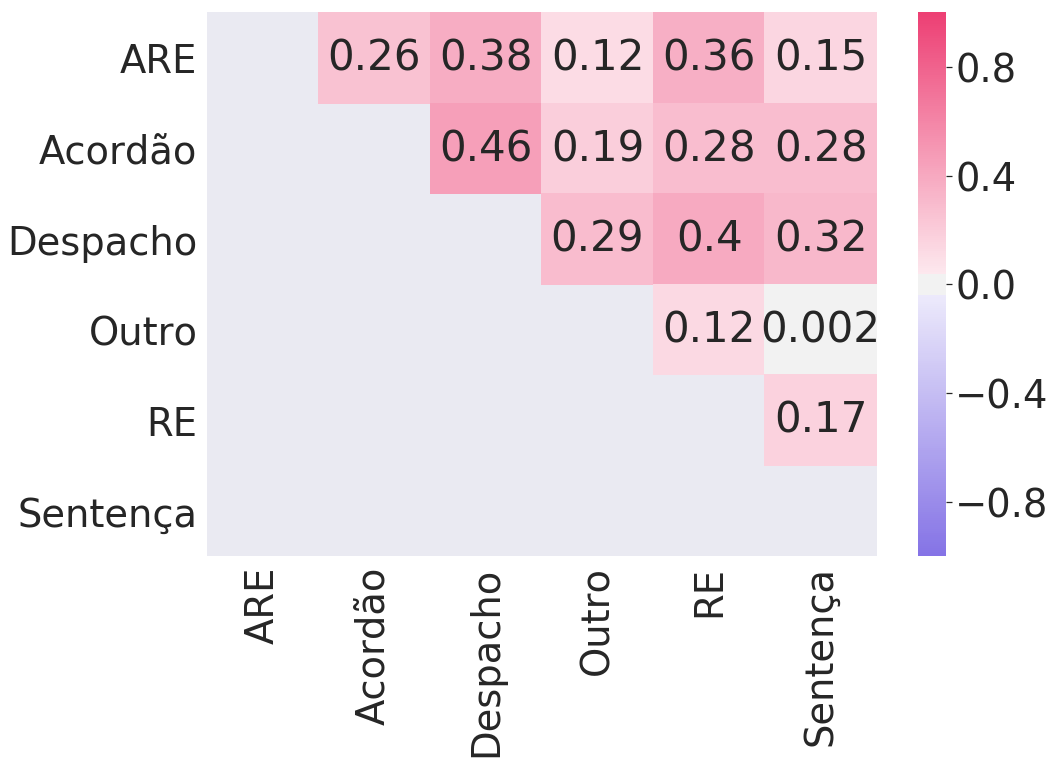
\includegraphics[width=\textwidth]{figuras/precorr}
        \caption{Correlação do texto com pré-processamento}
    \end{subfigure}
    \caption[Mapa de calor para correlação entre peças]{Mapa de calor para correlação entre os tipos peças. Fonte: GPAM \protect\footnotemark}
  \label{fig:correlacaoPecas}
\end{figure}

\footnotetext{O Grupo de Pesquisa em Aprendizado de Máquina (GPAM) <http://gpam.unb.br/> está envolvido na tarefa de classificar peças para o STF. Esta imagem foi gerada para a exploração de dados realizada no projeto. Elaborado pelos membros: Davi Alves Bezerra e Davi Benevides Gusmão.}

% Utilizou-se a implementação do SVM Linear \cite{hearst_support_1998} para treinar com todos os dados, a fim de obter uma caracterização das palavras mais importantes. Os parâmetros utilizados foram os padrões de acordo com a implementação de \citeauthor{pedregosa_scikit-learn:_2011} (\citeyear{pedregosa_scikit-learn:_2011}), modificando apenas o número máximo de iterações para 50.000, pois somente com este valor que garantiu-se a convergência do modelo.

% \begin{figure}[h]
% 	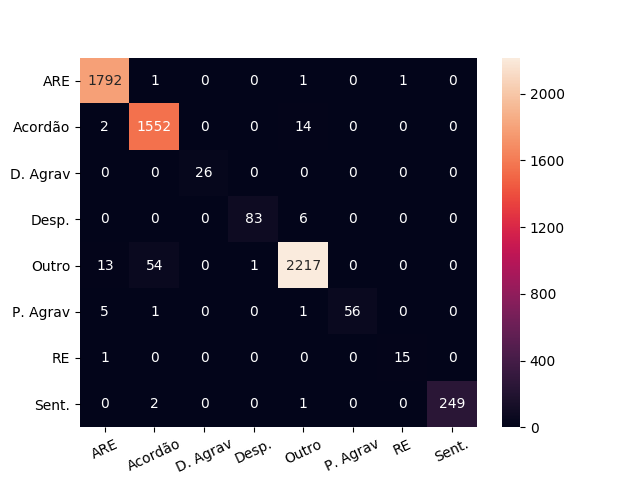
\includegraphics[keepaspectratio=true,scale=0.6]{figuras/confusionMatrixSMV}
%     \centering
% 	\caption[Matriz de confusão para extração de características usando SVM]{Matriz de confusão para extração de características usando SVM. Fonte: elaboração própria}
% 	\label{fig:svmDisperssao}
% \end{figure}

% A figura \ref{fig:svmDisperssao} mostra que o modelo conseguiu separar bem as peças, e portanto, a Tabela \ref{tab:caracteristicasImportantes} mostra as características mais importantes extraídas dos vetores de suporte \cite{hearst_support_1998}.

% Muitas palavras que não fazem sentido para o contexto do conteúdo das peças, como nomes próprios, apareceram de forma muito frequente durante a classificação (Exemplo: 'piauí', 'ubaldino', 'glacy', 'crisanto'). Apesar disso, as peças ARE, RE, Sentença e Despacho de Agravo mostraram palavras de importância significativas. Na tabela \ref{tab:caracteristicasImportantes}, as palavras relevantes de acordo com a Seção \ref{sec:cpc} estão em negrito.

% \begin{table}[h]
%   \centering
%   \caption[Características importantes extraídas dos vetores de suporte]{Características importantes extraídas dos vetores de suporte.}
%   \label{tab:caracteristicasImportantes}
%   \begin{tabular}{|p{1cm}|m{1.5cm}|m{1.5cm}|m{1.5cm}|m{1.5cm}|m{1.5cm}|m{1.5cm}|m{1.5cm}|m{1.5cm}|}
%   	\hline
% 	\textbf{Pos} & \textbf{Agr. RE} & \textbf{Acórdão} & \textbf{D. Agr.} & \textbf{Desp.} & \textbf{Outro} & \textbf{P. Agr.} & \textbf{RE} & \textbf{Sen- \newline tença} \\ \hline
% 	1 &  https & liar & monsani & marmelo & ubaldino & sulmar & \textbf{artigo\newline\_102} & montrazi \\ \hline
% 	2 &  \textbf{extraor-\newline dinário} & chegar & munici- \newline pio & rollin & sumie & glacy & \textbf{consti-\newline tuição} & \textbf{inspeção} \\ \hline
%     3 &  quintar & borrar & dezembro & amina- \newline dabe & minhos & bradesco & iii & \textbf{decidir} \\ \hline
%     4 &  bandeiro & pg & município & cear & membro & \textbf{ag} & presentar & requis \\ \hline
%     5 &  toste & piauí & vigência & spprev & crispin & vencedor & \textbf{venia} & \textbf{dispen- \newline sar} \\ \hline
%     6 &  muci- \newline ciaria & filhar & obser- \newline vância & previ- \newline dencia & rizar & marcar & objeto & \textbf{artigo \newline \_42} \\ \hline
%     7 &  unimed & \textbf{recurso} & \textbf{instru- \newline mentar} & líbero & parcial & \textbf{regi- \newline mental} & alínea & invalidez \\ \hline
%     8 &  \textbf{federar} & carrá & blumenau & cásper & cleci & sortear & \textbf{reper- \newline cussão} & \textbf{funda- \newline mentar} \\ \hline
%     9 &  acessar & unani- \newline midade & prever & itau & vanin & paraiba & incisar & moléstia \\ \hline
%     10 &  quo & universo & termo & \textbf{recu- \newline perar} & ller & crisanto & dispo- \newline sitivo & expor \\ \hline
%     11 & \textbf{juizado} & agostar & \textbf{lei \newline \_13256} & recupe- \newline ração & evori & ferrar & \textbf{recursal} & \textbf{postular} \\ \hline
%     12 &  novembro & batistuzo & \textbf{regi- \newline mental} & creditos & pastar & incs & respeito & \textbf{produzir} \\ \hline
%     13 &  diretoria & eichherr & assistir & fundação & especial & aguardar & presença & represen- \newline tante \\ \hline
%     14 &  denega- \newline tório & dezembro & recursais & pintar & \textbf{agravo} & pf & \textbf{juizados} & julga- \newline mento \\ \hline
%     15 &  trâmite & sangiogo & \textbf{presi- \newline dência} & represen- \newline tação & \textbf{artigo\newline \_48} & freuden- \newline thal & cabível & rocar \\ \hline
%     16 &  segurar & autoprev & base & artigo\newline\_25 & suprir & obrigação & taubaté & íntegro \\ \hline
%     17 &  eletroni- \newline camente & bitello & união & veiculos & \textbf{preâm- \newline bulo} & servidor & \textbf{razão} & capaci- \newline dade \\ \hline
%     18 &  enviar & entre- \newline tanto & alterar & mjr & \textbf{cnj} & paraíba & exa & \textbf{código} \\ \hline
%     19 &  \textbf{proces- \newline sual} & registrar & \textbf{lei\newline\_13105} & nelcis & paname- \newline ricano & efone & prolatado & intuito \\ \hline
%     20 &  \textbf{artigo\newline\_544} & sedi- \newline mentar & repúblico & quantum & despachar & \textbf{previsto} & egrégio & procu- \newline rador \\ \hline
%   \end{tabular}\par  Fonte: Elaboração própria.
% \end{table}